% !TEX root = ./cvl.tex
\section{Multi-scale filtering Problem}
\label{sec:background}

%\marcos{Here is where your basic definitions go, e.g., what is a cell, what are zoom levels, how are objects typically selected when creating a map, what are basic and implicit constraints, such as adjacency and zoom consistency, what are application-specific constraints, what is importance/weight, etc.}

In the multi-scale filtering problem we select the subsets of the dataset that should be displayed on each scale of the generated map. Below we define the basic components of the problem, and informally define the associated optimization problem. 

\subsection{Geospatial records and weights}
\label{sec:records}

% Definition records
% Weights

The dataset is assumed to consist of a set of \emph{geospatial records} that are drawn from a database table. Each record has a geometry, e.g.\ is a point, line segment, polygon --- or is a collection of simple geometric entities. Also, each geospatial record has relevant associated information, for example a city name, a hotel name or a description of an incident that took place at the given spatial location. Each record is assumed to have a unique ID.

Each record is assigned a \emph{user defined weight} using CVL (see Section~\ref{sec:cvl-language}). The weight represents the relative importance of a record in the generated map; an important (or highly ranked) record has a higher weight than a less important record. Any subset of records --- or all records for that matter --- may have the same weight. Therefore, the weights induce a partial order of the records.

%While the user does not need to individually assign weights to records, CVL offers a very flexible scheme for doing this. Weights are assigned by evaluating a SQL expression for each input row. For example a given column in the input database can be used directly as the weight of a record, or the length or area of the record geometry could be used. In fact any floating point expression can be used to weigh records, and it is perfectly ok to use the output of the random number generator or even a constant. 


\subsection{Zoom levels}
\label{sec:zoomlevels}

\marcos{I am wondering whether this section is about zoom levels, constraints, or zoom levels and constraints?}

% Scales and zoom levels
% Cells/tiles
% Density/visibility
% Proximity
% Zoom consistency

The map should be generated on multiple scales, as specified by the user. Let the zoom-levels run from 1 (lowest scale) to $\mathcal{Z}$ (largest scale). On a given zoom level, the map is rendered at a certain pixel resolution. Thus, for a given zoom level, we know the distance in pixels between geospatial locations. This gives rise to two fundamental constraints when generating a map for the dataset at a given zoom level.

\marcos{Why are these two constraints fundamental?}

Firstly, the principle of constant information density~\cite{topfer1966principles} implies that the number of records that can be displayed in an area of a certain pixel size should be bounded. Assume that we divide the complete map into cells (or tiles) of, say, 256 x 256 pixels. The \emph{density} constraint states that each cell can contain at most $K$ visible records, where $K$ is a user defined parameter.

\marcos{We use the term cellbound and also refer to visibility later in the paper. Should we introduce that nomenclature already here?}

Secondly, records cannot be too close to each other in the map --- otherwise the user will not be able to interactively manipulate records in the map. The \emph{proximity} constraint states that every pair of visible records must be separated by at least $d$ pixels, where $d$ is a user defined parameter.

In addition to these constraints that must hold separately for each zoom level, the filtering of the records must be consistent across zoom levels. The \emph{zoom-consistency} constraint~\cite{sarma2012fusiontables} states that when a record is filtered out at a given scale, it should also be filtered out at all \emph{lower} scales. When a user zooms out on a map, records can only disappear --- not reappear.

Apart from the zoom-consistency constraint which must hold for any map, the density and proximity constraints are optional. The user chooses the set of constraints that must hold for a given map, and can even define new constraints using the CVL language, see Section~\ref{sec:cvl-language}.

\subsection{Conflict sets and constraints}
\label{sec:conflicts}

\begin{figure}[htbp]
\begin{center}
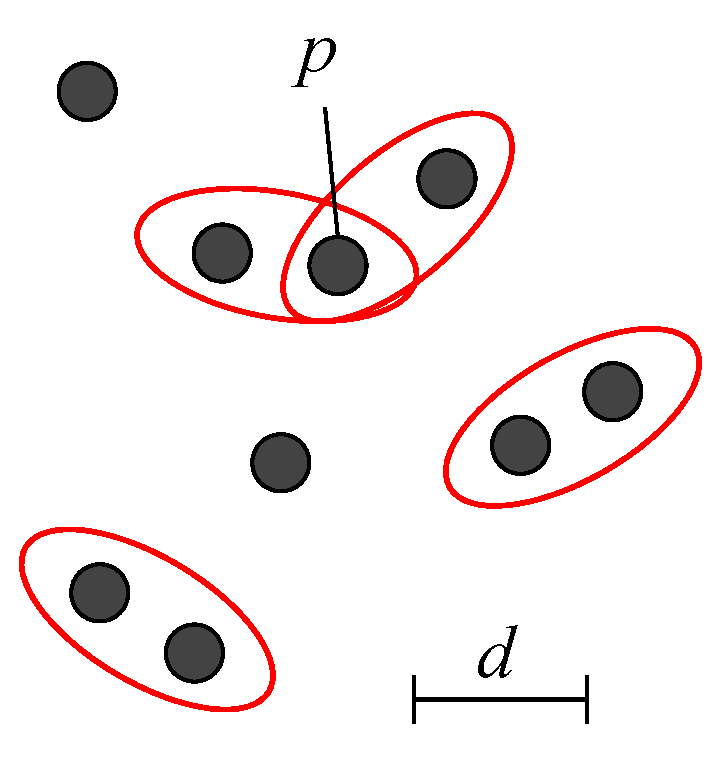
\includegraphics[scale=.4]{figs/cvl_proximity_conflicts.pdf}
\caption{Conflicts generated by the proximity constraint for distance $d$. Notice that point $p$ is a member of more than one conflict set.}
\label{fig:proximity:conflict}
\end{center}
\end{figure}

For a given zoom level, we model constraints such as density or proximity constraints using the notion of \emph{conflict sets}. A conflict set is a set of records that cannot all appear simultaneously at a given zoom level. For the density constraint, one conflict set is generated for each cell that contains more than $K$ records. For the proximity constraint, one conflict set is generated for each pair of records that is less than $d$ pixels apart. An example is shown in Figure~\ref{fig:proximity:conflict}. A record can be in several conflict sets, which is the case for point $p$ in the example.

Any cartographic constraint that can be formulated as a conflict set can be added by the user using CVL --- but this is also the only means of formulating constraints at a given zoom level. Thus in CVL there is a one-to-one correspondence between conflict sets and constraints. 

\marcos{If one CVL constraint generates multiple conflict sets, then how can there be a one-to-one correspondence between conflict sets and constraints?}

Consider a conflict set containing $k_1$ records, where at most $k_2$ of these records can appear on the map (where $k_1 > k_2$). Then it is equivalent to state that at least $\lambda = k_1 - k_2$ of these records must be \emph{filtered out} at the given zoom level. In the mathematical formulation of the problem in Section~\ref{sec:optimizationmodel} we will use this alternative way to formulate constraints.

%A cartographic constraint in CVL is a condition that must hold for all subsets of a given size. Subsets of records for which the condition does not hold, are said to be in conflict. As part of formulating a constraint, the user writes SQL that finds conflicts for this constraint. Part of the CVL formulation of the proximity constraint is an SQL statement that finds all records that are too near each other at a given zoom-level. The contract between the user and the CVL framework is that the user code must generate $\langle cid, rid \rangle$ tuples that represent the conflict sets. The sematics are that $rid$ is the ID of a record which is a member of a conflict set uniquely identified by $cid$. As an example, the user code for the proximity constraint generates two tuples for each conflict found.

%An example of a cartographic constraint in CVL is the \emph{proximity constraint} which states that at all zoom-levels all visible records must be separated by at least $d$ pixels. CVL does not generally need the user to specify at which zoom-level a record is too close to other records, only what the user considers to be "too close". The formulation of the proximity constraint implies that at each zoom-level a (possibly empty) subset of records must be removed in order to respect the constraint, and this is a general property of constraints in CVL. Which records are prioritized over others is controlled by assigning weights to records to indicate their importance. The implicit goal of evaluating a CVL query is to maintaining as much aggregate weight at each zoom-level as possible while satisfying all constraints.

%Rule-based languages like Styled Layer Descriptor (SLD)  and Mapnik XML serve a similar purpose as CVL, but using a different approach. The user explicitly decides the filtering of records at each zoom level and how records are presented. CVL is only concerned with the filtering, but is implicit about the exact zoom-level at which a record will appear.


\subsection{Filtering as an optimization problem}
\label{sec:filtering}

The overall task of multi-scale filtering is to identify a subset of the dataset at each zoom-level, such that all constraints are satisfied, and such that the aggregate weight of records that are removed is minimized. Note that if a record is filtered out at, say, 7 zoom levels, then the record contributes to the aggregate weight 7 times its user defined weight (the record must necessarily be filtered out at the lowest 7 zoom levels due to the zoom-consistence constraint). In this manner, filtering out high-weight records at high zoom levels is particularly costly --- which is exactly what we would like to achieve. In Section~\ref{sec:optimizationmodel} we present a mathematical formulation of this optimization problem.

%For example, if two records constitute a conflict with respect to the proximity constraint, the CVL framework will delete the one with lesser weight, unless deleting the record with higher weight yields are better global solution for that zoom-level. In other words, the user does not control directly how the framework resolves conflicts, but influences the decision by assigning record weights. 

%Given the set of conflict tuples generated by the user constraint code, the framework must decide how to resolve the conflicts. A conflict in CVL can always be resolved by removing a subset of the constituent records from the given zoom-level. How many records needs to be removed is also specified in the user code together with the code that finds the conflicts. For the proximity constraint we have to delete one record to resolve each conflict. How this is defined as user code is explained in Section~\ref{sec:create-constraint-statement}.

%\marcos{While I can certainly see that WMS@GST uses the process above, it is not clear that the three steps above are an accurate representation of all map services?}
%\marcos{It seems to me that it is important to say that rendering is orthogonal to the work, and that the selection task of generalization is computationally intensive and can be done at indexing time. Perhaps these two points can be conveyed with less words than in the section above and the section below? That would leave us space to introduce other important basic definitions listed in the comment at the beginning of this section.}

% text is moved to introduction /MZ
